    \documentclass[11pt,
        usenames, % allows access to some tikz colors
        dvipsnames % more colors: https://en.wikibooks.org/wiki/LaTeX/Colors
    ]{report}
    \usepackage{
        amsmath,
        amssymb,
        fouriernc, % fourier font w/ new century book
        fancyhdr, % page styling
        lastpage, % footer fanciness
        hyperref, % various links
        setspace, % line spacing
        amsthm, % newtheorem and proof environment
        mathtools, % \Aboxed for boxing inside aligns, among others
        float, % Allow [H] figure env alignment
        enumerate, % Allow custom enumerate numbering
        graphicx, % allow includegraphics with more filetypes
        wasysym, % \smiley!
        upgreek, % \upmu for \mum macro
        listings, % writing TrueType fonts and including code prettily
        tikz, % drawing things
        booktabs, % \bottomrule instead of hline apparently
        cancel % can cancel things out!
    }
    \usepackage[margin=1in]{geometry} % page geometry
    \usepackage[
        labelfont=bf, % caption names are labeled in bold
        font=scriptsize % smaller font for captions
    ]{caption}
    \usepackage[font=scriptsize]{subcaption} % subfigures

    \newcommand*{\scinot}[2]{#1\times10^{#2}}
    \newcommand*{\dotp}[2]{\left<#1\,\middle|\,#2\right>}
    \newcommand*{\rd}[2]{\frac{\mathrm{d}#1}{\mathrm{d}#2}}
    \newcommand*{\pd}[2]{\frac{\partial#1}{\partial#2}}
    \newcommand*{\rtd}[2]{\frac{\mathrm{d}^2#1}{\mathrm{d}#2^2}}
    \newcommand*{\ptd}[2]{\frac{\partial^2 #1}{\partial#2^2}}
    \newcommand*{\md}[2]{\frac{\mathrm{D}#1}{\mathrm{D}#2}}
    \newcommand*{\pvec}[1]{\vec{#1}^{\,\prime}}
    \newcommand*{\svec}[1]{\vec{#1}\;\!}
    \newcommand*{\bm}[1]{\boldsymbol{\mathbf{#1}}}
    \newcommand*{\ang}[0]{\;\text{\AA}}
    \newcommand*{\mum}[0]{\;\upmu \mathrm{m}}
    \newcommand*{\at}[1]{\left.#1\right|}

    \newtheorem{theorem}{Theorem}[section]

    \let\Re\undefined
    \let\Im\undefined
    \DeclareMathOperator{\Res}{Res}
    \DeclareMathOperator{\Re}{Re}
    \DeclareMathOperator{\Im}{Im}
    \DeclareMathOperator{\Log}{Log}
    \DeclareMathOperator{\Arg}{Arg}
    \DeclareMathOperator{\Tr}{Tr}
    \DeclareMathOperator{\E}{E}
    \DeclareMathOperator{\Var}{Var}
    \DeclareMathOperator*{\argmin}{argmin}
    \DeclareMathOperator*{\argmax}{argmax}
    \DeclareMathOperator{\sgn}{sgn}
    \DeclareMathOperator{\diag}{diag\;}

    \DeclarePairedDelimiter\bra{\langle}{\rvert}
    \DeclarePairedDelimiter\ket{\lvert}{\rangle}
    \DeclarePairedDelimiter\abs{\lvert}{\rvert}
    \DeclarePairedDelimiter\ev{\langle}{\rangle}
    \DeclarePairedDelimiter\p{\lparen}{\rparen}
    \DeclarePairedDelimiter\s{\lbrack}{\rbrack}
    \DeclarePairedDelimiter\z{\lbrace}{\rbrace}

    % \everymath{\displaystyle} % biggify limits of inline sums and integrals
    \tikzstyle{circ} % usage: \node[circ, placement] (label) {text};
        = [draw, circle, fill=white, node distance=3cm, minimum height=2em]
    \definecolor{commentgreen}{rgb}{0,0.6,0}
    \lstset{
        basicstyle=\ttfamily\footnotesize,
        frame=single,
        numbers=left,
        showstringspaces=false,
        keywordstyle=\color{blue},
        stringstyle=\color{purple},
        commentstyle=\color{commentgreen},
        morecomment=[l][\color{magenta}]{\#}
    }

\begin{document}

\def\Snospace~{\S{}} % hack to remove the space left after autorefs
\renewcommand*{\sectionautorefname}{\Snospace}
\renewcommand*{\appendixautorefname}{\Snospace}
\renewcommand*{\figureautorefname}{Fig.}
\renewcommand*{\equationautorefname}{Eq.}
\renewcommand*{\tableautorefname}{Tab.}

\onehalfspacing

\pagestyle{fancy}
\rfoot{Yubo Su}
\cfoot{\thepage/\pageref{LastPage}}

\title{Research Notes}
\author{Yubo Su}
\rhead{}

\maketitle

\tableofcontents

\newpage

\chapter{Preliminary Problems}

To get an intuition for how Dedalus and fluid mechanics works, we will solve
some toy problems. Recall fluid equations in the presence of a uniform
gravitational field $\vec{g} = -g\hat{z}$:
\begin{equation}
    \begin{split}
        \pd{\rho}{t} + \vec{\nabla} \cdot \p*{\rho \vec{u}} &= 0,\\
        \rd{\vec{u}}{t} + \frac{\vec{\nabla}P}{\rho} - \vec{g} &= 0.
    \end{split}\label{eq:fluid_eq}
\end{equation}

In the incompressible limit, $\rd{\rho}{t} = 0$, which implies $\vec{\nabla}
\cdot \vec{u} = 0$. We use subscripts to indicate perturbed quantities, $Q_0$ is
background and $Q_1$ is perturbed. We will generally use $\vec{u}_0 = 0$ unless
otherwise noted. We will also generally assume symmetry along all axes except
$z$ the vertical axis.

In the incompressible limit, the fluid equations become
\begin{equation}
    \begin{split}
        \vec{\nabla} \cdot \vec{u}_1 &= 0,\\
        \pd{\rho_1}{t} + u_{1z}\pd{\rho_0}{z} &= 0,\\
        \pd{\vec{u}_1}{t} + \frac{1}{\rho_0}\vec{\nabla}P_1
            + \frac{\rho_1 g \hat{z}}{\rho_0} &= 0.
    \end{split}\label{eq:lin.incomp}
\end{equation}
We have used $\vec{\nabla}P_0 = -\rho_0 g \hat{z}$ in the absence of
perturbations.

\section{Incompressible, No Gravity}

We note that in the no gravity limit that $\rho_1$ does not have an effect on
other dynamical variables, so the equations of motion we must solve are
\begin{equation}
    \begin{split}
        \vec{\nabla} \cdot \vec{u}_1 &= 0,\\
        \pd{\vec{u}_1}{t} + \frac{\vec{\nabla}P_1}{\rho_0} &= 0.
    \end{split}\label{eq:lin.no_g_eom}
\end{equation}
We can take the divergence of the momentum equation and substitute the
continuity equation to get $\nabla^2 P = 0$.

\subsection{Dirichlet BCs}

This is a Laplace equation, which we've solved countless times. Imposing
periodic boundary conditions in the $x$ direction and $P_1(z = L) = 0, P_1(z =
0) = \mathcal{P}(x, t)$, we obtain eigenfunctions
\begin{equation}
    \begin{split}
        P_{1, n}(x, z, t) &=
            \frac{\mathcal{P}_n(t)}{\sinh(k_nL)}e^{ik_nx}\sinh\p*{k_n(L - z)},\\
        u_{1x, n}(x, z, t) &=
            \int\limits^t -\frac{1}{\rho_0}\pd{P_{1, n}}{x}\;\mathrm{d}t,\\
        u_{1z, n}(x, z, t) &=
            \int\limits^t -\frac{1}{\rho_0}\pd{P_{1, n}}{z}\;\mathrm{d}t.
    \end{split}\label{eq:incomp_nog}
\end{equation}
We define $k_n = \frac{2\pi n}{L}, n \geq 0$ and $\mathcal{P}(x, t) =
\sum\limits_n \mathcal{P}_n(t)e^{ik_nx}$.

Thus, if we impose BCs $\mathcal{P}(x, t) = \sin \frac{2\pi x}{L}$ and start
with initial conditions such that all quantities are zero, we would expect after
transients die out that
\begin{equation}
    \begin{split}
        P(x, z, t) &= \frac{\sin \frac{2\pi x}{L}}{\sinh 2\pi}
            \sinh \p*{2\pi \frac{L - z}{L}},\\
        u_{1x}(x, z, t) &= -\frac{2\pi t}{L\rho_0}
            \frac{\cos \frac{2\pi x}{L}}{\sinh 2\pi}\sinh \p*{2\pi \frac{L -
                z}{L}},\\
        u_{1z}(x, z, t) &= +\frac{2\pi t}{L\rho_0}
            \frac{\sin \frac{2\pi z}{L}}{\sinh 2\pi}\cosh \p*{2\pi \frac{L -
                z}{L}}.
    \end{split}\label{eq:incomp_nog_sol}
\end{equation}
This is in good agreement with the results, presented in \autoref{fig:no_g}.
Note that $P$ is constant while $\vec{u}$ increases linearly in time, and we
observe the expected $\sim \sin x \sinh \frac{L - z}{z}$ dependence. In fact,
$u_{1x}, u_{1z}$ are exactly $\frac{2\pi}{10}$ at $t = 1$.
\begin{figure}[!h]
    \centering
    \begin{subfigure}{0.3\textwidth}
        \centering
        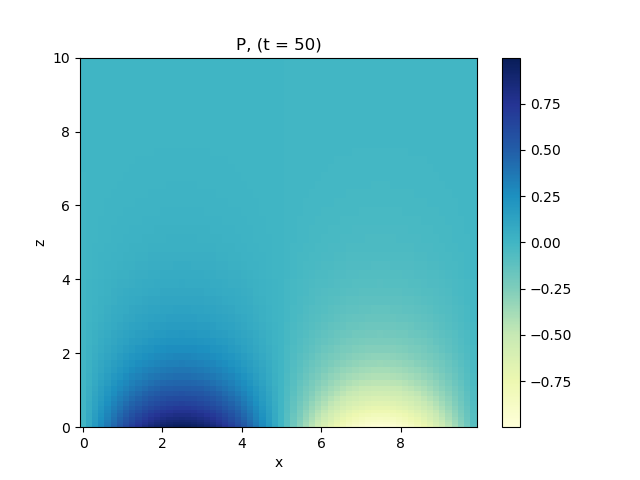
\includegraphics[width=\textwidth]{../sims_old/2d_0_no_g/no_g_P_t50.png}
    \end{subfigure}
    \begin{subfigure}{0.3\textwidth}
        \centering
        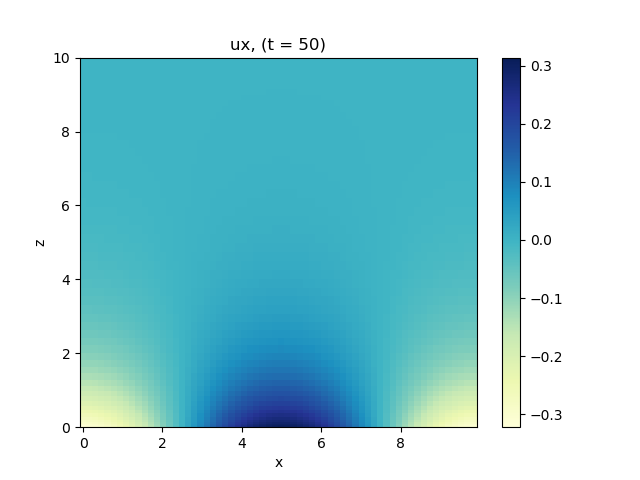
\includegraphics[width=\textwidth]{../sims_old/2d_0_no_g/no_g_ux_t50.png}
    \end{subfigure}
    \begin{subfigure}{0.3\textwidth}
        \centering
        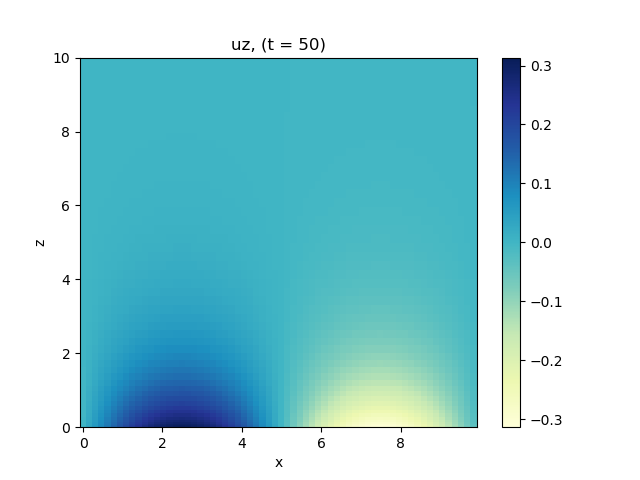
\includegraphics[width=\textwidth]{../sims_old/2d_0_no_g/no_g_uz_t50.png}
    \end{subfigure}

    \begin{subfigure}{0.3\textwidth}
        \centering
        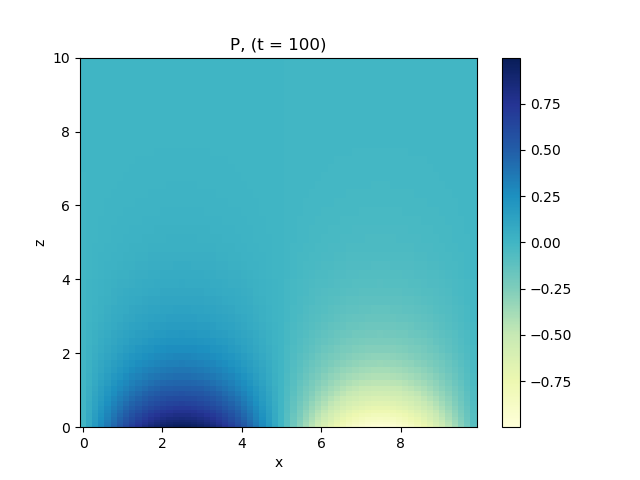
\includegraphics[width=\textwidth]{../sims_old/2d_0_no_g/no_g_P_t100.png}
    \end{subfigure}
    \begin{subfigure}{0.3\textwidth}
        \centering
        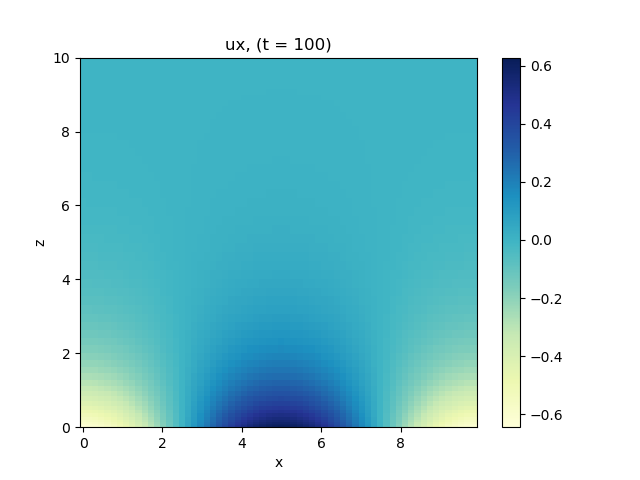
\includegraphics[width=\textwidth]{../sims_old/2d_0_no_g/no_g_ux_t100.png}
    \end{subfigure}
    \begin{subfigure}{0.3\textwidth}
        \centering
        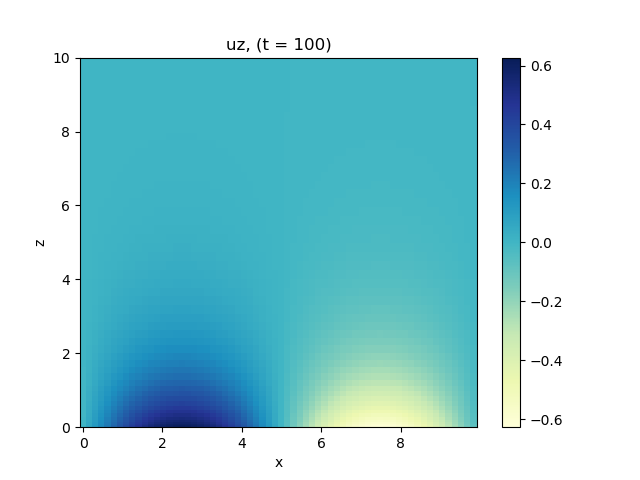
\includegraphics[width=\textwidth]{../sims_old/2d_0_no_g/no_g_uz_t100.png}
    \end{subfigure}
    \caption{$P, u_x, u_z$ at $t = 0.5$ and $t = 1$ for $\rho_0 = 1$. We choose
    a $L = 10$ square domain.}\label{fig:no_g}
\end{figure}

\subsection{Things to Note}

It is worth noting that, since our \autoref{eq:lin.no_g_eom} reduced to a Laplace
equation, we needed two $z$ BCs and two $x$ BCs (periodic BCs amount to equating
the value and derivative of the function). This is in agreement with the
observation that the original \autoref{eq:lin.no_g_eom} had two derivatives in
$x, z$ apiece, so we needed two BCs each.

It is also worth seeing from our solution that $P$ immediately goes to the
equilibrium solution. This is not surprising since in the incompressible limit,
sound speed goes to infinity which is the timescale on which the pressure field
adjusts to net forces. Thus, the dynamics solely arise from the static pressure
field pushing the velocity field to equilibrium.

We chose time-independent $\mathcal{P}(x, t)$, but it is clear that whatever
$\mathcal{P}(x, t)$ we choose, the time dependence propagates to the velocities
by way of an integral. If we had instead chosen to take Fourier transform $t \to
\omega$, we would have had to integrate the boundary condition against the
eigenfunctions for each of the $\omega$, which is still easily computable, to
get the full $u_{1x}(x, z, t)$. We consider this in preparation for when we can
only solve for a set of $\vec{k}, \omega$ in the next problem.

The next thing we would have wanted to do is solve a problem with radiative BCs,
but we need to have wave solutions, which are missing in the absence of gravity.
We thus move on to the next configuration.

\section{Incompressible, Stratified w/ Gravity}

\subsection{Eigenfunctions}

Let's restore the $\rho_1 g$ term now. For funsies, we begin by solving for
arbitrary stratification $\rho_0(z)$ first. The fluid equations to first order
reduce to
\begin{equation}
    \begin{split}
        \pd{\rho_1}{t} + \vec{u}_1 \cdot \p*{\vec{\nabla}\rho_0} &= 0,\\
        \vec{\nabla} \cdot \vec{u}_1 &= 0,\\
        \pd{\vec{u}_1}{t} &= -\frac{\vec{\nabla}P_1}{\rho_0}
            - \frac{\rho_1 g}{\rho_0}
    \end{split}\label{eq:lin_incomp}
\end{equation}
We expect there to be some $z$ dependence in the amplitude, so we substitute
variables of form $e^{i(kx - \omega t)}$ and do not specify the $z$ dependence.
This gives us
\begin{equation}
    \begin{split}
        -i\omega \rho_1 - u_{1z}\pd{\rho_0}{z} &= 0,\\
        iku_{1x} + \pd{u_{1z}}{z} &= 0,\\
        -iw u_{1x} + \frac{ik_x P_1}{\rho_0} &= 0,\\
        -iw u_{1z} + \frac{1}{\rho_0}\pd{P_1}{z} +
            \frac{\rho_1 g}{\rho_g} &= 0.
    \end{split}
\end{equation}
We substitute $N^2 = -\frac{g}{\rho_0}\pd{\rho_0}{z}$ to obtain
\begin{subequations}
    \begin{align}
        -i\omega \rho_1 - u_{1z}\frac{\rho_0N^2}{g} &= 0,\label{eq:lin.cont}\\
        iku_{1x} + \pd{u_{1z}}{z} &= 0,\label{eq:lin.div}\\
        -iw u_{1x} + \frac{ik_x P_1}{\rho_0} &= 0,\label{eq:lin.mom_x}\\
        -iw u_{1z} + \frac{1}{\rho_0}\pd{P_1}{z} +
            \frac{\rho_1g}{\rho_0} &= 0.\label{eq:lin.mom_z}
    \end{align}
\end{subequations}
Eliminating $u_{1x}$ by substituting~\eqref{eq:lin.div}
into~\eqref{eq:lin.mom_x} and $\rho_1$ by substituting~\eqref{eq:lin.cont}
into~\eqref{eq:lin.mom_z} give
\begin{subequations}
    \begin{align}
        i\omega \pd{u_{1z}}{z} + \frac{k_x^2 P_1}{\rho_0} &= 0,
            \label{eq:lin.eq1}\\
        \p*{\omega^2 - N^2 }u_{1z} + \frac{i\omega}{\rho_0}\pd{P_1}{z} &= 0.
            \label{eq:lin.eq2}
    \end{align}
\end{subequations}
Finally, we multiply~\eqref{eq:lin.eq1} with $\rho_0$ and differentiate
$\mathrm{d}z$ and combine with~\eqref{eq:lin.eq2} to give
\begin{equation}
    \rtd{u_{1z}}{z} + \frac{1}{\rho_0}\pd{\rho_0}{z}\pd{u_{1z}}{z}
        + k_x^2\p*{\frac{N^2}{\omega^2} - 1}u_{1z} = 0.\label{eq:lin.incomp.gen}
\end{equation}

Let's now pick stratification $\rho \propto e^{-z/H}$
\autoref{eq:lin.incomp.gen} clearly has exponential solutions $e^{\kappa z}$ for
\begin{equation}
    \kappa^2 - \frac{\kappa}{H} + k_x^2\p*{\frac{N^2}{\omega^2} - 1} = 0.
\end{equation}
We permit complex $\kappa = \frac{1}{2H} + ik_z$, and from the above clearly
\begin{align}
    k_z^2 &= -\frac{1}{4H^2} + k_x^2\p*{\frac{N^2}{\omega^2} - 1},\nonumber\\
    \omega^2 &= \frac{N^2k_x^2}{k_x^2 + k_z^2 +
        \frac{1}{4H^2}}.\label{eq:strat_disp}
\end{align}
Thus the eigenfunctions are
\begin{equation}
    \begin{split}
        u_{1z} &= e^{z/2H} e^{i(k_zz + k_xx - \omega t)},\\
        u_{1x} &= -\frac{k_z + i/2H}{k_x} u_{1z},\\
        \rho_1 &= \frac{i \rho_0}{H\omega} u_{1z},\\
        P_1 &= -\frac{\rho_0 \omega}{k_x^2}\p*{k_z + i/2H}u_{1z}.
    \end{split}\label{eq:strat_eigens}
\end{equation}

\subsection{Analytically Solving an IVP, Dirichlet + Driving BCs}

We will analyze everything in terms of $u_{1z}$ since it has the simplest form;
note that when actually choosing the BCs we will have to consider the gauge
freedom of $P$ and some considerations we defer to the computational section.

Currently, we have a set of eigenfunctions
\begin{equation}
    u_{1z}\p*{x, z, t \middle| \vec{k}, \omega}
        = e^{z/2H} e^{i(k_zz + k_xx - \omega t)}.
        \label{eq:strat.uz_eigen}
\end{equation}
Note that $u_{1z}$ is really only a function of two parameters rather than the
three $(k_x, k_z, \omega)$, since the three are related by dispersion relation
\autoref{eq:strat_disp}.

Now, we implement BCs. Consider domain $x, z \in [0, L]$. We will use periodic
BCs again in $x$, so then $k_{x, n} = \frac{2\pi n}{L}, n \geq 0$. Then, we will
require $u_{1z, n}(x, L, t) = 0$, a Dirichlet condition at the top boundary,
which restricts us to eigenfunctions of form
\begin{equation}
    u_{1z, n}\p*{x, z, t \middle| \vec{k}, \omega}
        = e^{z/2H}e^{i(k_xx - \omega t)}\sin\p*{k_z\p*{L - z}}.
        \label{eq:strat.uz_eigen_l-z}
\end{equation}

Finally, we must choose a BC at $z = 0$. We will choose a general function
$u_{1z}(x, 0, t) = F(x, t)$ where we can decompose
\begin{equation}
    F(x, t) = \int\limits \sum\limits_n \mathcal{F}(k_{x, n}, \omega)
        e^{i(k_{x, n}x - \omega t)}\;\mathrm{d}\omega.
\end{equation}
Matching BCs then gives us general solution for $u_{1z}$ given an arbitrary
driving function
\begin{equation}
    u_{1z}\p*{x, z, t \middle| \vec{k}, \omega}
        = \int\limits \sum\limits_n \mathcal{F}\p*{k_{x, n}, \omega}
            \frac{e^{z/2H}e^{i\p*{k_{x, n}x - \omega t}}\sin \p*{k_z(L - z)}}{
            \sin k_zL}\;\mathrm{d}\omega.
            \label{eq:strat.full_sol}
\end{equation}

For ease of computation, let's pick $F(x, t) = \cos \p*{\frac{2 \pi x}{L} -
\omega_0 t}$, so our full expected solution is (note $A + \epsilon =
Ae^{\epsilon/A} + \mathcal{O}(\epsilon^2)$)
\begin{equation}
    \begin{split}
        u_{1z}\p*{x, z, t \middle | \vec{k}, \omega}
            &= e^{z/2H}\frac{\cos\p*{\frac{2\pi x}{L} - \omega_0 t}
                \sin \p*{k_z(L - z)}}{\sin k_zL},\\
        u_{1x}\p*{x, z, t \middle | \vec{k}, \omega}
            &\approx \frac{k_z}{k_x} e^{z/2H}\frac{
                \cos\p*{\frac{2\pi x}{L} - \omega_0 t + \frac{1}{2Hk_z}}
                \sin \p*{k_z(L - z)}
            }{\sin k_zL},\\
        \rho_1\p*{x, z, t \middle | \vec{k}, \omega}
            &\approx \frac{\rho_0}{H\omega} e^{z/2H}\frac{
                -\sin\p*{\frac{2\pi x}{L} - \omega_0 t}
                \sin \p*{k_z(L - z)}
            }{\sin k_zL},\\
        P_1\p*{x, z, t \middle | \vec{k}, \omega}
            &\approx -\frac{\rho_0 \omega k_z}{k_x^2} e^{z/2H}\frac{
                \cos\p*{\frac{2\pi x}{L} - \omega_0 t + \frac{1}{2Hk_z}}
                \sin \p*{k_z(L - z)}
            }{\sin k_zL},\\
    \end{split}\label{eq:strat.part_sol}
\end{equation}
where $k_z: \omega(k_x, k_z) = \omega_0$ by the dispersion relation
\autoref{eq:strat_disp}. Note that $H$ contributes both to the overall
exponential profile and to the phase lag of $u_{1x}$.

\subsection{Computationally Solving an IVP, Dirichlet + Driving BCs}

To solve this computationally with the aforementioned BCs, periodic in $x$,
Dirichlet $0$ at $z = L$ and $\cos \p*{\frac{2\pi x}{L} - \omega_0 t}$ at $z =
0$, we must address the gauge freedom in $P$. This arises because for $k_x = 0$,
the divergence-free condition $\vec{\nabla} \cdot \vec{u}_1 = \pd{u_z}{z} = 0$
specificies $u_{1z}$ up to a constant already, so the bottom BC will fix the
value of $u_z$ when $k_x = 0$.

A different way of phrasing the same argument is as follows. Consider the
discrete $N \times N$ (square for notational simplicity) grid. At the boundary,
there is a list of values $f\p*{\z*{x_i}, z_0}$ that lives in an $N$ dimensional
space. We can thus pick a spanning set of $N$ basis vectors, and for each of
these $N$ vectors, by enforcing $\vec{\nabla} \cdot \vec{u} = 0$ at the boundary
we fix the allowed $f\p*{\z*{x_i}, z_{-1}}$ boundary conditions we can implement.
But there exists a choice of basis vectors for which one of the basis vectors is
constant $f_i\p*{\z*{x_i}, z_0} = C$. For this basis vector, the boundary
condition is fully determined, so we only have $N - 1$ dimensions from which to
choose the BCs $f\p*{\z*{x_i}, z_{-1}}$. Since the dimensionality of a space
cannot depend on the choice of basis vector, the divergence free condition
actually yields an extra degree of freedom.

We can use this extra degreee of freedom to specify $P(z = L) = 0$ so the
oscillations should have zero mean. Then we can just simulate away!

From here we can just tweak the parameters until we get something useful, can
look at the videos. Note that we should simulate until at least $T >
\frac{2L_z}{v_{p, z}}$ the $z$ phase space velocity, so we can capture any
reflections off the boundary. Turns out both Dirichlet and Neumann BCs give
strong reflections that produce standing waves in the $z$ and traveling waves in
the $x$.

\subsection{Phase/Group Velocity}

Let's figure out the analytical forms for the phase, group velocity and the
energy density/power flux.

Let's first consider the phase velocity. We traditionally think about the phase
velocity in 1D $v_{ph} = \frac{\omega(k)}{k}$, but in general it is the function
such that $\vec{k} \cdot \vec{r} - \omega t = \vec{k} \cdot \p*{\vec{r} -
\vec{v}_{ph}t}$ is constant (the phase of the wave). Thus, it must satisfy
$\vec{k} \cdot \vec{v}_{ph} = \omega$, and so one sensible choice is
\begin{equation}
    \vec{v}_{ph} = \frac{\omega \hat{k}}{\abs{\vec{k}}}
        = \frac{\omega \vec{k}}{\abs{\vec{k}}^2}.
        \label{eq:v_ph}
\end{equation}

For our stratified atmosphere problem, $\omega^2 = \frac{N^2 k_x^2}{k^2 +
\frac{1}{4H^2}}$. This corresponds to $\vec{v}_{ph} = \frac{Nk_x}{\sqrt{k_x^2 +
k_z^2 + 1/4H^2}} \vec{k}$.

On the other hand the group velocity is given $\vec{v}_g =
\pd{\omega}{k_i}\hat{\imath}$. In our problem, $v_{g, z} =
-\frac{Nk_xk_z}{\p*{k_x^2 + k_z^2 + 1/4H^2}^{3/2}}$ while $v_{g, x} =
\frac{N}{\sqrt{k_x^2 + k_z^2 + 1/4H^2}} - \frac{Nk_x^2}{\p*{k_x^2 +
k_z^2 + 1/4H^2}^{3/2}} = \frac{N\p*{k_z^2 + 1/4H^2}}{\p*{k_x^2 +
k_z^2 + 1/4H^2}^{3/2}}$.

\subsection{Energy/Power Flux}

To compute the energy and power flux of the wave, we recall that for a general
fluid the energy conservation equation reads
\begin{equation}
    \pd{}{t}\p*{\frac{1}{2}\rho v^2 + \rho \epsilon}
        = \vec{\nabla} \cdot \p*{
            \rho \vec{v}\p*{v^2 + \epsilon + \frac{P}{\rho}}
        },
\end{equation}
where $\epsilon$ is the internal energy. But since $P = (\gamma -
1)\rho\epsilon$ and we take $\gamma \to \infty$ incompressible limit, $\epsilon
= 0$, so the energy of the wave is just $\frac{1}{2}\p*{\rho_0 + \rho_1} u_1^2$
and the power flux is $\p*{\rho_0 + \rho_1}\vec{u}_1u_1^2 + P_1\vec{u}_1$.

Another formula given by Sutherland 2011 is $\pd{\ev*{E}}{t} = v_{g, z}
\ev*{E}$ where we average over $x$ one wavelength. I wasn't able to show
that these two agree in general; Sutherland's formula seems to be derived for a
traveling wavepacket whereas we have no such thing. We do not use this
expression since the Landau \& Lifshitz expression works well.

\section{Supressing Reflection}

Sourced from \url{https://people.maths.ox.ac.uk/trefethen/6all.pdf}. There are
largely two ways to do this. The first is to add a damping zone, a region in
which $\dot{q} = -q/\tau_d(z)$ where $\tau_d(0) = 0$ and increases to some
non-small number for some $z_0$ beyond which we want damping. One form, chosen
in Ryan and Dong's paper, is to use multiplicative factor $f(z) = \max\s*{0, 1 -
\frac{\p*{z - z_b}^2}{\p*{z_d - z_b}^2}}$ where $z_b$ is where one begins
supression and $z_b$ is the boundary. Then a dynamical variable $q$ can be
supressed via $\dot{q} = (\dots) - f(z)\frac{q - q_0}{\tau}$ where $\tau$ is the
dynamical timescale on which to damp and $q_0$ is the value to damp to. We will
apply this only to the velocity variables with an eye to extending this approach
to the nonlinear regime, where the velocity variables should still be damped to
zero but $\rho, P$ must capture the stratification and so cannot easily be
artificially damped (maybe? Revisit if this does poorly compared to damping all
linear variables, and damp the nonlinear variables to their
equilibrium/stratified values).

\subsection{First Order}

In order to compute the reflecting boundary condition, we must find a
sequence of differential operators that well approxmiates the system of PDEs. We
can get this from the dispersion relation; since our radiating boundary is along
$z$, we should try to solve for $k_z$ in the dispersion relation to get a
pseudodifferential operator form for $\pd{}{z}u_z$ (we take $k_xH \ll 1$ as well
to simplify):
\begin{align}
    k_z^2 &= \frac{N^2}{\omega^2}k_x^2 - k_x^2 - \frac{1}{4H^2},\nonumber\\
        &\approx k_x^2\p*{\frac{N^2}{\omega^2} - 1},\\
    \pd{u_z}{z} &\approx -\pd{u_z}{x}\sqrt{\frac{N^2}{\omega^2} - 1}.
\end{align}
We pick the negative sign in accordance with an outgoing wave, per the group
velocity formulae for $k_z > k_x$.

From the numerical simulations, it is clear that reflections are well supressed
initially, but the the simulation blows up. This is because our supression is
imperfect (differential approximation to a pseudodifferential operator) and
since our system is dissipation free, reflection grows. Moreover, since any
reflected components seem to have different $k_x, k_z, \omega$, the second time
they're incident on the boundary, our above condition becomes wildly inaccurate.

\section{The Difficulty of the Incompressible, Nonlinear Problem}

We consider the problem where both advective terms are kept and $\rho_1 \sim
\rho_0$. We write down thus nonlinear fluid equations
\begin{equation}
    \begin{split}
        \pd{\rho}{t} + \vec{u} \cdot \p*{\vec{\nabla}\rho} &= 0,\\
        \vec{\nabla} \cdot \vec{u} &= 0,\\
        \pd{\vec{u}}{t} &= -\p*{\vec{u} \cdot \vec{\nabla}} \vec{u}
            - \frac{\vec{\nabla}P}{\rho} - g\hat{z}.
    \end{split}\label{eq:nonlin_incomp}
\end{equation}
Note that we cannot even subtract off hydrostatic equilibrium anymore since
$\rho$ can deviate greatly from the normal $\rho_0e^{-z/H}$!

\subsection{Rearrangement for Dedalus}

In order to simulate this at all in a spectral program, recall the way that
nonlinear PDEs are decomposed in a spectral code. Given a phase space $Q$,
consider first a system of PDEs expressible in form
\begin{equation}
    \dot{Q} + \bm{L}Q + f(Q) = g
\end{equation}
where $\dot{Q}$ is the time derivative, $\bm{L}$ is some linear operator, $f(Q)$
are nonlinear terms and $g$ is an arbitrary driving function. Spectral codes
work by re-casting the operators to be purely algebraic in an appropriate
spectral basis consisting of some $\varphi_i$ trial and $\xi_i$ test functions.
The \emph{tau spectral method} that Dedalus uses considers using the trial
functions as the test functions, so the effective decomposition that is
performed is
\begin{equation}
    \bra*{\varphi_i}\dot{Q} + \bm{L}Q \ket*{\varphi_j}
        = \dot{Q}_i + L_{ij}Q_q = \bra*{\varphi_i}-f(Q)  + g \ket*{\varphi_i}.
\end{equation}
It is then clear that $-f(Q) + g$ can just be treated as inhomogeneous source
terms, and over a short $\Delta t$ it can be approximated via $-f(Q_0) + g$.
This first-order inhomegeneous ODE then admits closed form exact solutions
$e^{-L_{ij}t}\p*{\dots}$.

One can imagine, for this matter, that $\pd{}{t}$ can be wrapped in the $L_{ij}$
operator and the timestepping computed implicitly; I believe this is what
Dedalus does, implicitly timestepping the left hand side and explicitly the
inhomogeneous terms.

Both of these procedures require $\bm{L}$ linear operator or $\pd{}{t} + \bm{L}$
to be full rank, or invertible. This is enforced analytically by requiring the
same number of BCs as derivatives, and numerically this is little different.
This is why it is possible to have components of $Q$ that are not differentiated
$\partial_t$ but still have well-defined time evolutions; the only condition
required is that the linear terms of the PDE make up a full-rank operator.
Hence, in our linear incompressible equations, we permitted use of $\vec{\nabla}
\cdot \vec{u}_1 = 0$ in lieu of a $\pd{P}{t}$ explicit equation of motion; so
long as the gauge for $P$ (which only appears in derivatives) is properly set,
the operator is full rank and numerically well-defined.

In the case of the full nonlinear equations though, it bears noting that $P$
only appears in nonlinear terms! Thus, the linear terms clearly cannot have full
rank since they fail to reference $P$ at all. We remedy this by re-casting the
momentum equation as
\begin{equation}
    \pd{\vec{u}}{t} + \frac{\vec{\nabla}P}{\rho_0}
        = -\vec{\nabla}P\p*{\frac{1}{\rho} - \frac{1}{\rho_0}}
            + \vec{g}.
\end{equation}
This ensures that, along with suitable gauge choice for $P$, the linear
operators on the left hand side of the equation have full rank. The remaining
equations
\begin{subequations}
    \begin{align}
        \pd{\rho}{t} &= -\vec{u} \cdot \vec{\nabla}\rho,\\
        \vec{\nabla} \cdot \vec{u} &= 0,
    \end{align}
\end{subequations}
remain unchanged.

\subsection{Pathology with $u_z$ BCs}

Our problem turns out to be ill-conditioned, the pathology arising from our
driving term in conjunction with the incompressibility constraint. Since we want
to model the propagation of waves from where they are excited, rather than
exciting them directly in our problem, we must drive our region of interest via
boundary conditions rather than forcing terms.

By driving via boundary conditions, we can only specify boundary conditions on
the variables being differentiated $\partial_z$ in our equations of motion,
since we enforce fully periodic BCs in $x$ via using a Fourier spectral
decomposition. Thus, we are restricted to enforcing BCs on either $\vec{u}$ or
$P$.

It turns out that by using BCs on $\vec{u}$, we run into a problem: the BCs we
specify on $u_z$ or its derivatives will in general affect grid points
$\partial_z u_{z, 1x}$ while those specified on $u_x$ can only affect
$\partial_x u_{x, 0x}$. This means that $\partial_x u_x$ will pick up
sharp jerks by being coupled to the BC, producing high frequency components in
$u_x$ as can be seen in \autoref{fig:agree_plots}. These come from enforcing the
divergence-free condition too literally at the boundary. Not that the figure was
produced with only a Dirichlet BC on $u_z$, no BCs on $u_x$, in a linear system
with absorbing BCs.
\begin{figure}[!h]
    \centering
    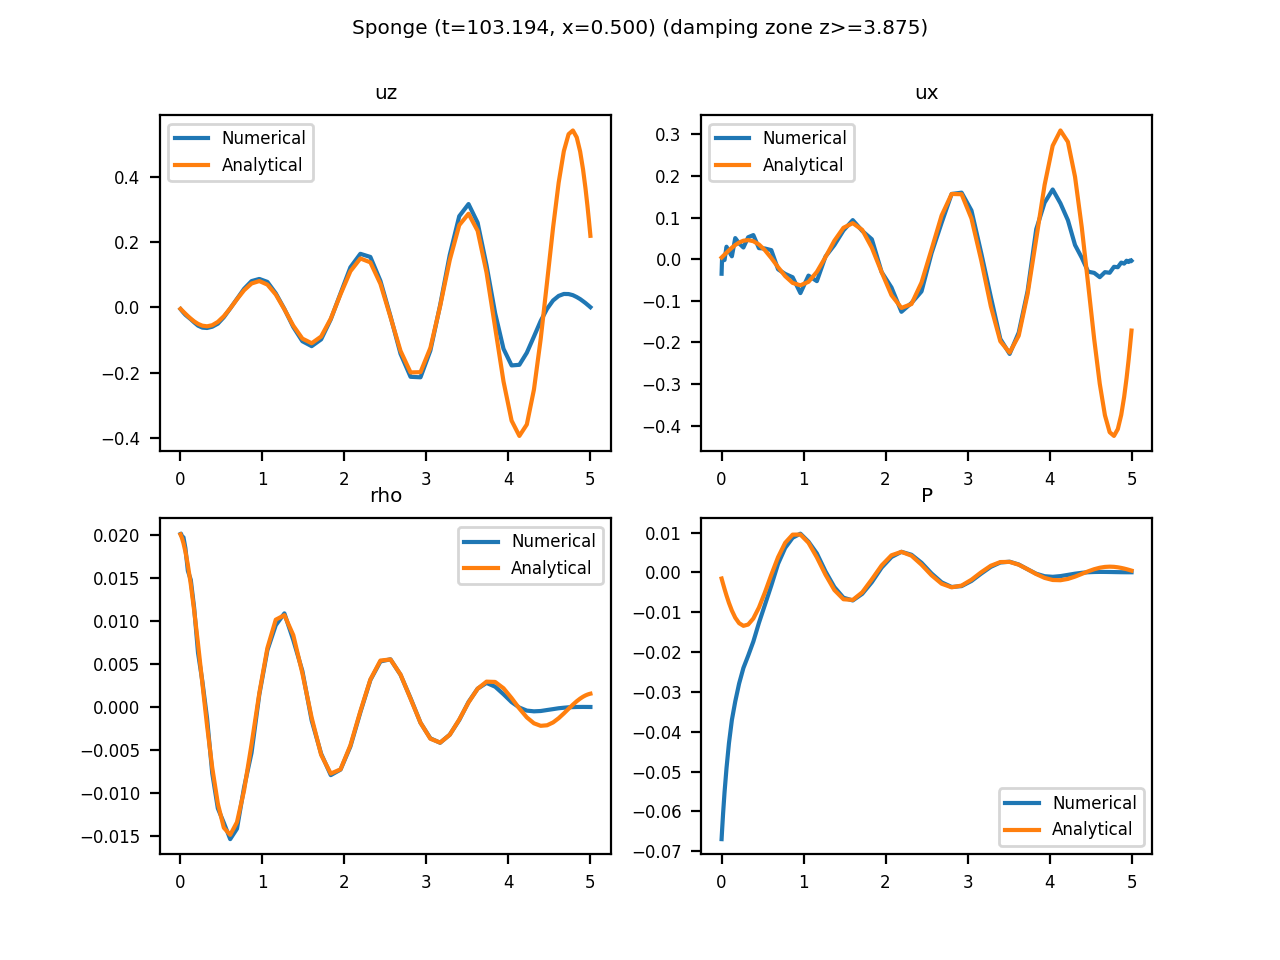
\includegraphics[width=0.7\textwidth]{../sims_old/2d_1_strat/agree_plots/sponge_2.png}
    \caption{Note the jaggedness in $u_x$ induced by a Dirichlet BC on
    $u_z$.}\label{fig:agree_plots}
\end{figure}

This problem seems to be remedied somewhat by instead enforcing Neumann BCs on
$u_z$, or even when allowing dissipation enforcing Neumann BCs on $\partial_z
u_z$ (the extra derivatives granted by $\nu \nabla^2 \vec{u}$ let us specify
higher order BCs). However, in the fully nonlinear system we still observe
divergences near $z=0$ regardless of how smooth of BCs we use on $u_z$.
Moreover, since the discontinuities come from the nature of the BC and not its
strength, we run into these instabilities regardless of how gradually we
introduce the BC (e.g.\ we could consider multiplying by $1 - e^{-t/\tau}$ to
gradually introduce the BC, but this turns out also to be unstable).

There are thus three possible solutions to this:
\begin{itemize}
    \item Consider BCs only on $P$, the only other choice of dynamical variable.
        This seems to also exhibit instabilities near $z = 0$.

    \item Consider using a $\nabla^2 P$ equation instead of a $\vec{\nabla}
        \cdot \vec{u} = 0$ constraint. The correct choice of BCs in this case is
        discussed in Nordstrom et al, 2006. We choose not to investigate this.

    \item Change the system of equations to no longer consider an incompressible
        system; the anelastic system is an attractive alternative. This boasts
        the advantage of not having an algebraic constraint equation.
\end{itemize}

TODO Can taking $\rho_1 \ll \rho_0$, giving us a full rank operator w/o doing
the janky double add thing, solve in the incompressible limit? Otherwise, go
anelastic.

\section{Limits of the Incompressibility and Anelasticity Assumptions}

To get a better handle on the regimes of validity of the incompressible and
anelastic approximations, we return to the full fluid equations
\begin{equation}
    \begin{split}
        \pd{\rho}{t} + \vec{\nabla} \cdot \p*{\rho \vec{u}} &= 0,\\
        \pd{\vec{u}}{t} + \p*{\vec{u} \cdot \vec{\nabla}}\vec{u} +
            \frac{\vec{\nabla}P}{\rho} - \vec{g} &= 0.
    \end{split}
\end{equation}
Furthermore, we assume small perturbations $\delta P = c_s^2 \delta \rho$ where
$c_s^2$ is the sound speed, also the velocity at which an adiabatic perturbation
is restored. We drop the $-\vec{g}$ from the analysis assuming that it is
largely negated by an appropriate background $P$.

Given these considerations, we consider in what limit we may presume the fluid
to be incompressible. Consider if $\abs*{\vec{u}} \ll c_s$, then for some
characteristic frequency $\omega$ and wavenumber $k$ the momentum equation
scales as $\omega u + ku^2 + c_s^2 \delta \rho/\rho = 0$. Comparing scales it is
thus clear that $\delta \rho \ll \rho$ in this limit. Then, considering the
mass continuity equation, we recognize that the scalings are $\omega \delta \rho
+ \rho \vec{\nabla} \cdot \vec{u} + k\delta \rho u = 0$. Thus, $\vec{\nabla}
\cdot \vec{u} = 0$ necessarily, since $\rho$ is much larger than the other two
terms, and we obtain the incompressible mass continuity equation from the other
two terms. While this is obviously not a very careful treatment, it should
suffice to convince us that $u \ll c, \delta \rho \ll \rho, \vec{\nabla} \cdot
\vec{u} = 0$ are all roughly equivalent conditions.

On the other hand, when may we drop the total derivative terms? This seems to be
a slightly different criterion, and indeed we may compare $\pd{\vec{u}}{t} +
\p*{\vec{u} \cdot \vec{\nabla}} \vec{u} \sim \omega \vec{u} + ku^2$. Thus, the
second term is dominated by the first term when $\vec{u} \ll \vec{v}_{ph}$ where
$\vec{v}_{ph} \equiv \frac{\omega}{k}\hat{k}$ is the phase velocity. Recall that
for our stratified waves that $\omega \leq N = \sqrt{g/H}$ as a point of
reference. So we require $u \ll v_{ph}$ to be able to drop the total derivative
terms.

Since in general $v_{ph} \ll c_s$, we thus identify that there are three
regimes. The first, $u \ll v_{ph}$, we solve the completely linear problem.
Then, for $v_{ph} \lesssim u \ll c_s$, we must begin to consider the advective
terms but are still allowed to assume $\rho_1 \ll \rho_0$, an assumption that is
only violated when $u \sim c_s$.

If we look ahead to the anelastic system derivation, we can identify that the
anelastic approximation corresponds to assuming $c_s^2 \gg uv_{ph}$, making no
assertion of the scale between $u, v_{ph}$. Thus, we can also consider the
anelastic approximation with advective terms just fine in teh regime $v_{ph}
\lesssim u$, and if this is sufficient to induce wave breaking then we may never
need to consider the $\rho_1 \sim \rho_0$ enormous perturbations.

\chapter{Simulation Setup}

We describe now some concerns that arise in setting up the simulation.

\section{Damping Zone}

Since our code is a spectral code, instead of using the quadratic damping zone
presented from before (whose second derivative is discontinuous over the entire
domain), we prefer instead an $\arctan$ profile, such that
\begin{equation}
    \Gamma(z) \propto 0.5 * \p*{
        2 + \tanh C\p*{\frac{z - z_t}{L_z - z_t}}
            + \tanh C\p*{\frac{z - z_b}{z_b}}}.
\end{equation}
This is a profile that mostly vanishes $z \in [z_b, z_t]$ but is unity for $z
\lesssim z_b, z \gtrsim z_t$, with steepness of transition governed by factor
$C$. While this profile may have reflection issues if $C$ is chosen to be too
steep, it is smooth and so has exponentially convergent spectral expansion and
empirically seems to do alright.

It is moreover prudent to note that, since implicit calculations are expensive,
as long as the damping timescale $\Gamma^{-1}$ is everywhere resolved it is
cheaper to put $\Gamma \rho_1, \Gamma \vec{u}_1$ on the right hand sides of
their equations in Dedalus, which is timestepped explicitly.

\section{Volumetric Forcing}

Due to the structure of \lstinline{Dedalus}, we must use Chebyshev polynomials
in the vertical direction (to be able to enforce BCs). But as discussed in
\autoref{s:chebyshev}, the grid spacing of the Chebyshev polynomials near
boundaries goes as $1/N^2$, which means that interface forcing necessitates an
extremely strict Courant condition to capture evolution near the interface; this
is the explanation for the divergences we were seeing in earlier sections. In
fact, in the literature, the spectral CFL condition meets a $\Delta t_{\max}
\sim 1/N^2$ scaling thanks to poor bounds near the boundary.

Instead, we employ volumetric forcing. As a toy problem of seeing how this
works, we will study the restricted 1D wave equation.

\subsection{1D Wave Equation (Deprecated)}

Consider the forced 1D wave equation (we set $c = 1$)
\begin{equation}
    \ptd{u(x, t)}{t} - \ptd{u(x, t)}{x} = f(x, t).
\end{equation}
Note that the only allowed propagation modes here are $u \sim e^{iC\p*{x \pm
t}}$ for some constant $C$.

We wish to choose $f(x, t)$ such that $u\p*{x \to -\infty} = 0$ while $u\p*{x
\to +\infty} \sim e^{i\p*{x - t}}$. It is clear that if we consider the Fourier
transform $\tilde{f}(k, t)$, the response in $\tilde{u}(k, t)$ will also contain
components for each of the nonzero $\tilde{f}(k, t)$ components. Thus, if we
want a pure $e^{i(x - t)}$ outgoing wave, we should have a pure $\tilde{f}(k, t)
\propto \delta\p*{k - 1}$. However, it is clear that driving the oscillator
exactly on resonance produces divergent oscillation amplitudes, and moreover it
is impossible to drive with an $f(x, t)$ that doesn't vanish as $x \to \pm
\infty$.

It is nonetheless clear that $\tilde{f}(k, t)$ should be strongly peaked at $k =
1$ and small elsewhere. We can thus consider a form $f(x, t) \propto
e^{-x^2/2\sigma^2} e^{i(x - t)}$ such that $\sigma \gg 1$, i.e.\ the envelope
contains many wavelengths. The Fourier transform $\tilde{f}(k, t)$ is then a
Gaussian with width $1/\sigma \ll 1$ centered at $k = 1$ (convolution).

More precisely, consider $f(x, t) = f_0e^{-x^2/2\sigma^2} e^{i(x - t)}$ and $u(x,
t) = u_0(x)e^{i(x - t)}$ such that $u_0(x \to \infty) = 0$. Substituting this
into the inhomogeneous PDE gives
\begin{equation}
    i\pd{u_0(x)}{x} - \ptd{u_0(x)}{x} = f_0e^{-x^2/2\sigma^2}.
\end{equation}
We note that if $\sigma \gg 1$ then roughly $\pd{}{x} \ll 1$ or
\begin{equation}
    \pd{u_0(x)}{x} \approx -if_0e^{-x^2/2\sigma^2}.
\end{equation}
Enforcing $u_0(x \to -\infty) = 0$, then $\abs*{u_0(x \to +\infty)} =
f_0\sigma\sqrt{2\pi}$.

\subsection{Narrow-band forcing}

Instead of doing this on-frequency forcing, we choose instead to use a narrow
forcing zone $f(x, t) \sim N_{\sigma}(z)e^{it}$ where $\sigma$ is not large.
Specifically, we need $\sigma$ to be well-resolved spectrally, but we need
$\tilde{f}(k_z, t)$ not to be small. Thus, since $1/k_z$ must be resolved by the
simulation, choosing $\sigma = 1/k_z$ is a natural choice.

Note that this implies that waves will be excited going both upwards and
downwards, as $\tilde{f}(k_z) = \tilde{f}(-k_z)$. We can however place the
forcing zone near the bottom boundary so that downwards-propagating waves will
be attenuated by damping zones.

Let us derive the resultant equations of motion. In the interest of maintaining
a divergence-free velocity field, we place the driving term on the density
equation. Since the forcing is purely to excite waves and not physical (for the
time being), it should not worry us that driving the density equation is
ill-justifiable physically.

Consider the linearized system of equations (to examine the excited perturbation
in the linear legime)
\begin{subequations}\label{se:vol_drive}
    \begin{align}
        \vec{\nabla} \cdot \vec{u} &= 0,\\
        \pd{\vec{u}_1}{t} + \frac{\vec{\nabla}P}{\rho_0}
            + \frac{\rho_1 \vec{g}}{\rho_0}
            &= 0,\\
        \pd{\rho_1}{t} - \frac{u_{1z} \rho_0}{H}
            &= F(x, z, t),\\
        F(x, z, t) &= \Re Fe^{-\frac{(z - z_0)^2}{2\sigma^2}}
            e^{i\p*{k_xx - \omega t}}.
    \end{align}
\end{subequations}
For the linearized system, we can immediately substitute $\pd{}{t} \to -i\omega,
\pd{}{x} \to ik_x$, giving
\begin{align*}
    \pd{u_{1z}}{z} + ik_xu_x &= 0,\\
    -i\omega u_x + \frac{ik_xP}{\rho_0} &= 0,\\
    -i\omega u_{1z} + \frac{1}{\rho_0}\pd{P}{z} + \frac{\rho_1 g}{\rho_0} &= 0,\\
    -i\omega \rho_1 - \frac{u_{1z}\rho_0}{H} &= F.
\end{align*}
This can be recast solely in terms of $u_{1z}$ as
\begin{align*}
    -i\omega u_{1z} + \frac{\omega}{k_x}\p*{-\frac{1}{ik_x}\ptd{u_{1z}}{z}
        + \frac{1}{ik_xH}\pd{u_{1z}}{z}} - \frac{u_{1z}g}{Hi\omega}
        - \frac{Fg}{i\omega \rho_0} = 0,\\
    \omega^2\p*{
        k_x^2u_{1z} + \frac{1}{H}\pd{u_{1z}}{z} - \ptd{u_{1z}}{z}
    } - u_{1z}N^2k_x^2 - \frac{Fgk_x^2}{\rho_0} = 0.
\end{align*}
Note that if $\pd{}{z} \to 1/2H + ik_z, F = 0$ then this simplifies to the expected
dispersion relation $\omega^2 = \frac{N^2k_x^2}{k_x^2 + k_z^2 +
\frac{1}{4H^2}}$.

If we approximate $F(x, z, t) \approx F_0\delta\p*{z - z_0} e^{i(k_xx - \omega t)}$
for the time being, then clearly the only term that can be equally singular is
the $\ptd{}{z}$ term, leaving us with
\begin{equation}
    -\omega^2 \ptd{u_{1z}}{z} - \frac{Fgk_x^2}{\rho_0} = 0.
\end{equation}
Since $u_{1z}$ both above and below $z_0$ satisfy the homogeneous PDE, which has
plane wave solutions with an $e^{z/2H}$ envelope where $k_zH \gg 1$, we can
integrate about a small domain around $z_0$ and obtain
\begin{equation}
    \at{\pd{u_{1z}}{z}}_{z > z_0} - \at{\pd{u_{1z}}{z}}_{z < z_0}
        = -F_0\frac{gk_x^2}{\rho_0\omega^2}e^{i(k_xx - \omega t)}.
\end{equation}
It should then be apparent that the $u_{1z}$ solution is
\begin{equation}
    u_{1z} = \frac{F_0gk_x^2}{\rho_0(z = z_0)\omega^2}\frac{1}{2ik_z} \times
    \begin{cases}
        e^{(z - z_0)/2H}e^{i(k_xx + k_z(z - z_0) - \omega t)} & z > z_0\\
        e^{(z - z_0)/2H}e^{i(k_xx - k_z(z - z_0) - \omega t)} & z < z_0\\
    \end{cases}.
\end{equation}

Given that we are actually using a Gaussian $F(x, z, t) \propto F_0e^{-\frac{(z
- z_0)^2}{2\sigma^2}}$, the integral under $F(z)$ is actually
$F_0\sqrt{2\pi}\sigma$ rather than just $F_0$. Finally, since a delta function
is flat in spatial frequency space while a Gaussian tapers off with width
$1/\sigma$ ($\sigma$ is the spatial width, so $1/\sigma$ is the spatial
frequency width), we should expect an overall multiplicative factor of
$e^{-k_z^2\sigma^2 / 2}$ in the $k_z$ spatial component of $F(x, z, t)$ compared
to the delta function case. Thus, we finally obtain
\begin{equation}
    \abs*{u_{1z}(z = z_0)} = \frac{F_0\sqrt{2\pi}\sigma gk_x^2}{
        2\rho_0\p*{z = z_0}\omega^2 k_z}e^{-k_z^2\sigma^2/2}.
\end{equation}

\section{Timestepping}

\subsection{Signatures of Insufficient Temporal Resolution}

When running these simulations, it can occasionally be seen that the waves do
not grow in amplitude like $e^{z/2H}$, such that the energy and flux are not
constant (or the waves will grow too quickly; this is dependent on the exact
timestepping used). This is caused by using an overly-long timestep, as can be
seen with the below illustration.

We study the 1D advection equation $\psi_t = c\psi_x$ corresponding to
rightwards propagating waves. Consider first order implicit Euler timestepping
for wave mode $\psi_x = ik\psi$, then
\begin{equation}
    \psi_{i + 1} - \psi_i = ick\Delta t\psi_{i + 1}.
\end{equation}
Solving yields
\begin{align}
    \psi_{i + 1} &= \p*{1 - ick\Delta t}^{-1}\psi_i,\nonumber\\
        &= \p*{1 - i\omega \Delta t}^{-1}\psi_i.
\end{align}
If we then want to step forwards for some total time $T$, with $N \Delta t = T$
the number of timesteps taken, then we approximate
\begin{align}
    \psi(t_0 + T) \approx \p*{1 - i\omega \frac{T}{N}}^{-N}\psi(t_0).
\end{align}
It is worth noting that in the $N \to \infty$ limit we recover $\psi(t_0 + T) =
e^{i\omega T}\psi(t_0)$.

However, consider if $\omega \Delta t \lesssim 1$, then we should see the wave
amplitude decrease over time like
\begin{equation}
    \abs*{\psi(t_0 + T)} \approx \p*{1 + \omega^2 \Delta t^2}^{-N/2}\psi(t_0).
\end{equation}
Thus, since we have an implicit first order scheme, the wave amplitude
\emph{decreases} over time spuriously. An explicit method would produce an
increase, but \lstinline{Dedalus} uses implicit timestepping. The exact rate of
decrease depends on the timestepper used, but it is clear that $\omega \Delta t
\ll 1$ is necessary to avoid this spurious decrease (in numerics language, ``the
oscillation must be well-resolved'').

\section{Algebraic Manipulations}

\subsection{Factoring out the exponential dependence}

I've had to do this algebra too many times now, so let's just consider if we
factor out the $e^{z/2H}$ exponential scaling on the dynamical variables and the
$e^{-z/H}$ scaling on $\rho_0$. This leaves us with:
\begin{subequations}\label{se:nonlin_factored}
    \begin{align}
        \vec{\nabla} \cdot \vec{u}_1 + \frac{u_{1z}}{2H} &= 0,\\
        \pd{\rho_1}{t} - \frac{u_{1z} \rho_0}{H} &= -e^{z/2H}\s*{
            \p*{\vec{u}_1 \cdot \vec{\nabla} \rho_1} + \frac{u_{1z}\rho_1}{2H}
        },\\
        \pd{\vec{u}_1}{t} + \frac{\vec{\nabla}P}{\rho_0}
            + \frac{P}{2H\rho_0}\hat{z} + \frac{\rho_1\vec{g}}{\rho_0}
            &= -e^{z/2H}\s*{
            \p*{\vec{u} \cdot \vec{\nabla} \vec{u}_1}
                + \frac{u_{1z}\vec{u}_1}{2H}
        }.
    \end{align}
\end{subequations}
I'm too lazy to re-notate my variables, so all of them are constant amplitude
over $z$ now.

\chapter{Stability Analysis}

\section{Modulational Instability of NLSE}

We study the nonlinear Schr\"odinger Equation (NLSE)
\begin{equation}
    i\psi_t + \psi_{xx} + \nu \abs*{\psi}^2\psi = 0.
\end{equation}
Sutherland's paper demonstrates an interaction between the wave and the
wave-induced mean flow ($\propto \abs*{\psi}^2$) that reduces the IGW system to
the NLSE\@. Here we follow Whitham's textbook in rederiving the modulational
instability criterion.

Consider for some fixed value $k_0$, then the linear SE (LSE) admits a plane
wave solution $\psi = e^{i(k_0x - \omega(k_0)t)}$ for some dispersion relation
$\omega(k)$. If instead we permit $\psi$ to be distributed in frequency space
near $k_0$, then we may notate
\begin{equation}
    \psi = \psi_0 \varphi = e^{i(k_0x - \omega(k_0) t)} \int\limits
        \exp\s*{i\p*{k' x - k'\pd{\omega}{k}t -
            \frac{1}{2}k'^2 \ptd{\omega}{k}t}}\;\mathrm{d}k',
\end{equation}
where $k' = k - k_0$ denotes the deviation from the central $k_0$
wavenumber. Defining $\omega' = \omega - \omega_0$, we may observe
\begin{equation}
    \omega' = k' \pd{\omega}{k} + \frac{1}{2}k'^2 \ptd{\omega}{k}.
\end{equation}
Making correspondence $-i\omega' \to \partial_t, ik' \to \partial_x$, we see
that $\varphi$ obeys dispersion relation
\begin{equation}
    i\p*{\varphi_t + \pd{\omega}{k}\varphi_x}
        + \frac{1}{2}\ptd{\omega}{k}\varphi_{xx} = 0.
\end{equation}
Thus, the modulation $\varphi$ translates at the group velocity, and we find
that $\varphi$ obeys a modified LSE in a comoving frame.

If we reintroduce the nonlinearity, we observe that $\nu \abs*{\psi}^2\psi = \nu
\abs*{\varphi}^2 \psi_0\varphi$, and so the nonlinearity modifies the LSE as
\begin{align}
    i\p*{\varphi_t + \pd{\omega}{k}\varphi_x}
        + \frac{1}{2}\ptd{\omega}{k}\varphi_{xx}
        + \nu \abs*{\varphi^2}\varphi &= 0,\\
    \omega' = k' \pd{\omega}{k} + \frac{1}{2}k'^2 \ptd{\omega}{k}
        - \nu a^2.\label{eq:nlse_disp}
\end{align}

Armed with this dispersion relation, we can apply the method of characteristics
to the system of equations describing any wavetrain
\begin{subequations}\label{eq:wavetrain}
    \begin{align}
        \pd{k}{t} + \pd{\omega}{x} &= 0,\label{eq:wavetrain_1}\\
        \pd{A^2}{t} + \pd{}{x}\p*{c_gA^2} &= 0.\label{eq:wavetrain_2}
    \end{align}
\end{subequations}
We denote $A$ the wave amplitude and $c_g$ the group velocity. In a nonlinear
system, $\omega = \omega(A, k)$, and to leading order in $A$ we expect $\omega =
\omega_0 + \omega_2A^2$, i.e.\ the dispersion should not depend on the sign of
$A$. Thus we may rewrite \autoref{eq:wavetrain} as
\begin{subequations}\label{eq:wavetrain_mod}
    \begin{align}
        \pd{k}{t} + \p*{\pd{\omega_{0}}{k} + \pd{\omega_2}{k}A^2}\pd{k}{x}
            + \omega_2 \pd{A^2}{x} &= 0,\\
        \pd{A^2}{t} + \pd{A^2}{x}\pd{\omega_0}{k} + A^2\ptd{\omega_0}{k}\pd{k}{x}
            &= 0.
    \end{align}
\end{subequations}
We first note that, in $A \to 0$, the equations decouple and both equations
describe propagation at the group velocity (they are already in characteristic
form $Q_{,t} + cQ_{,x} = 0$). With some foresight, we anticipate that the
$\pd{A^2}{x}$ term in the first equation will provide a $\mathcal{O}(A)$
correction to the group velocity, while the $\pd{\omega_2}{k}A^2\pd{k}{x}$ term
provides an $\mathcal{O}(A^2)$ correction, so we drop it.

The method of characteristics then requires we seek linear combinations of the
two equations such that all equations are in characteristic form. The Whitham
prescription says that if the original system is of form $A_{ij}q_{j, t} +
B_{ij}q_{j, x} = 0$, then the characteristic curves $X(T)$ satisfy $A_{ij}X +
B_{ij}T = 0$. Here, this yields
\begin{equation}
    X(T) = \p*{\pd{\omega_0}{k} \pm A\sqrt{\omega_2 \ptd{\omega_0}{k}}}T.
\end{equation}

Comparing to the NLSE dispersion relation \autoref{eq:nlse_disp}, we identify
that $\sqrt{-\nu \ptd{\omega_0}{k}}A$ is the correction to the group velocity.
Thus, if $\nu\ptd{\omega_0}{k} > 0$, we obtain a \emph{complex} group velocity,
which is identified with \emph{modulational instability}. Naively, this might
imply a steepening $k = c_{g, 0}t - i\sqrt{\nu\omega_0''}At$ with timescale
$\Gamma \sim \p*{A^2\nu\omega_0''}^{-1/2}$.

\chapter{Stratified Flow}

\section{Linear Equations}

We largely follow Booker \& Bretherton from 1966 though do not adopt the
Boussinesq approximation. Consider background shear flow $\vec{u}_0 =
u_0(z)\hat{x}$ and vertical stratification $\rho_0 \propto e^{-z/H}$, then
\begin{subequations}\label{se:shear_eq}
    \begin{align}
        \vec{\nabla} \cdot \vec{u}_1 &= 0,\\
        \pd{\rho_1}{t} + \p*{\vec{u} \cdot \vec{\nabla}}\rho_1
            - u_{1z}\frac{\rho_0}{H} &= 0,\\
        \pd{u_{1x}}{t} + \p*{\vec{u} \cdot \vec{\nabla}}\p*{u_{1x} + u_0}
            + \frac{1}{\rho_0}\pd{P}{x} &= 0,\\
        \pd{u_{1z}}{t} + \p*{\vec{u} \cdot \vec{\nabla}}u_{1z}
            + \frac{1}{\rho_0}\pd{P}{z} + \frac{\rho_1 g}{\rho_0} &= 0.
    \end{align}
\end{subequations}
Note that $\vec{u} \cdot \vec{\nabla} = \p*{\vec{u}_0 + \vec{u}_1} \cdot
\vec{\nabla}$.

We again assume plane waves in $x, t$ such that $u_{1z}(x, z, t) =
u_{1z}(z)e^{i(k_xx - \omega t)}$. We bracket second-order terms below and set
them to zero in the ensuing calculations
\begin{subequations}
    \begin{align}
        \pd{u_{1z}}{z} + ik_xu_{1x} &= 0,\\
        -i\omega \rho_1 + u_0ik_x\rho_1
            - u_{1z}\frac{\rho_0}{H}
            + \s*{\p*{\vec{u}_1 \cdot \vec{\nabla}} \rho_1} &= 0,\\
        -i\omega u_{1x} + u_0ik_x u_{1x}
            + \frac{1}{\rho_0}ik_xP + u_{1z}\pd{u_0}{z}
            + \s*{\vec{u}_1 \cdot \vec{\nabla} u_{1x}} &= 0,\\
        -i\omega u_{1z} + u_0ik_x u_{1z}
            + \frac{1}{\rho_0}\pd{P}{z} + \frac{\rho_1 g}{\rho_0}
            + \s*{\vec{u}_1 \cdot \vec{\nabla} u_{1z}} &= 0.\\
    \end{align}
\end{subequations}
Denote $\omega_{cr}(z) = \omega - u_0(z)k_x$ the corotating frequency. Using
then that $u_{1x} = \frac{i}{k_x}\pd{u_{1z}}{z}$, $\rho_1 = \frac{i
\rho_0}{H\omega_{cr}} u_{1z}$ and $P = \s*{i\omega_{cr}u_{1x} - u_{1z
\pd{u_0}{z}}} \frac{\rho_0}{ik_x}$, we can finally arrive at linearized equation
\begin{equation}
    \ptd{u_{1z}}{z} - \frac{1}{H}\pd{u_{1z}}{z} + \s*{
        \frac{k_x^2N^2}{\omega_{cr}^2}
            - k_x^2
            - \frac{k_x}{\omega_{cr}H}\pd{u_0}{z}
            + \frac{k_x}{\omega_{cr}} \ptd{u_0}{z}
    } u_{1z} = 0. \label{eq:shear_lin_uz}
\end{equation}
Note that if we make correspondences $ik_x \to \partial_x, i\omega_{cr} \to
\partial_t + u_0\partial_x$ and take $H \to \infty$ while holding $N^2$
constant, we recover Equation 2.1 of Booker \& Bretherton. We can also note that
if we take constant $u_0$ we recover the expected dispersion relation
\autoref{eq:strat_disp} for $\omega = \omega_{cr}$.

\section{Reflection/Transmission in Linear Theory}

One can solve \autoref{eq:shear_lin_uz} via \emph{Frobenius Theory}, but if we
consider only $\omega_{cr} \to 0$, we obtain a very simple power series
solution. In $\omega_{cr} \to 0$, we have only leading order contributions
\begin{equation}
    \ptd{u_{1z}}{z} + \frac{k_x^2N^2}{\omega_{cr}^2}u_{1z} = 0.
\end{equation}
Consider a power series solution $u_{1z} \propto \omega_{cr}^\alpha$, where
$\omega_{cr}(z) = \omega - k_xu_0(z)$. Note that very near the critical level,
$\pd{u_0}{z}\delta z k_x$ where $\delta z = z - z_c, \omega_{cr}(z_c) = 0$. We
thus have
\begin{align}
    \p*{\pd{\omega_{cr}}{z}}^2 \alpha\p*{\alpha - 1} + k_x^2N^2 &= 0,\\
    \alpha &= \frac{1}{2}\pm i\sqrt{\frac{N^2}{\p*{\pd{u_0}{z}}^2} -
        \frac{1}{4}}.
\end{align}
The classic Booker \& Bretherton paper notates this result $u_{1z} \propto
\p*{\omega_{cr}(z)}^{\frac{1}{2} \pm i\mu} \propto (\delta z)^{\frac{1}{2} \pm
i\mu}$.

Now, consistent with a perturbation that vanishes as $t \to -\infty$
(alternatively, this is just the Landau prescription for deforming below a
singularity on the real line), we must interpret $\omega_{cr}$ as having a
slight positive imaginary component. Given this, the expression for $u_{1z}(z)$
is multivalued, and we must specify a branch cut. For $\Arg\p*{z - z_c} = 0$, or
intuitively when we are above the critical layer, choose branch such that
\begin{equation}
    \p*{z - z_c}^{\frac{1}{2} \pm i\mu} \equiv
        \abs*{z - z_c}^{1/2\pm i\mu}.
\end{equation}
It is then clear that for $\Arg\p*{z - z_c} = -\pi$, intuitively corresponding
to being below the critical layer (note the arg is $-\pi$ since $z_c$ is
infinitesimally above the real axis), our branch cut enforces
\begin{equation}
    \p*{z - z_c}^{\frac{1}{2} \pm i\mu} =
        \abs*{z - z_c}^{\frac{1}{2} \pm i\mu}e^{-\frac{i\pi}{2}}e^{\mp \mu \pi}.
\end{equation}
Lastly, we interpret $\abs*{z - z_c}^{\pm i\mu} = e^{\pm i\mu \ln \abs*{z -
z_c}}$ to have the form of a positive/negative $k_z$ value. Interestingly, this
means that $e^{-i\mu \ln \abs*{z - z_c}}$ corresponds to the \emph{positive
group velocity}, which is $e^{\mu \pi}$ magnified compared to the $\Arg\p*{z -
z_c} = 0$ case, and $e^{2\mu \pi}$ magnified over the negative group velocity
component below $z_c$.

The interpretation we choose for this is that an incoming wavepacket moving with
positive group velocity inbound on $z_c$ is transmitted with amplitude $e^{-\mu
\pi}$ and reflected with amplitude $e^{-2\mu \pi}$. The remainder is interpreted
as being \emph{absorbed} by the critical layer.

\section{Validity of the Linear Approximation}

The real physics is expected to deviate from our computation near the critical
layer owing primarily to two effects: nonlinear advective terms and diffusivity.
Hazel 1967 found numerically that including diffusive tersm in the equations of
motion does not change the attenuation factor; even in the presence of
dissipation no reflection/transimission are observed. This makes sense;
examining the equations of motion, the effect of an extra $\pd{}{t} \to \pd{}{t}
- \nu \nabla^2$ is to take $\omega_{cr} \to \omega_{cr} + i\nu k_x^2 - i\nu
\ptd{}{z}$, giving the singularity at $\omega_{cr} + i\nu k_x^2 = 0$ the
positive imaginary component we before asserted.

On the other hand, other studies e.g.\ Brown \& Stewartson 1980, Winters \&
d'Asaro 1994, find that once the wave amplitude becomes nonnegligible, sizable
reflection can be found. In contrast, Ogilvie \& Barker 2010 find that in
geometrically focused breaking, no reflection is observed, despite the nonlinear
effects being stronger than the dissipitive ones. The study of how nonlinear and
diffusive effects compete is then nontrivial.

\clearpage

\appendix

\chapter{Deriving Fluids Results}

\section{Equation of Energy Conservation}

We follow Landau \& Lifshitz's derivation for this expression. Consider that the
total energy stored in a wave must be the sum of its kinetic and internal energy
$\frac{1}{2}\rho v^2 + \rho \epsilon$ where $\epsilon$ is the internal energy
density. To obtain an equation of energy conservation, we must take the time
derivative of this expression. First, we consider
\begin{align}
    \pd{}{t}\p*{\frac{1}{2}\rho v^2} &= \frac{1}{2}v^2\pd{\rho}{t}
        + \rho \vec{v} \cdot \pd{\vec{v}}{t},\nonumber\\
        &= -\frac{1}{2}v^2 \p*{\vec{\nabla} \cdot \rho \vec{v}}
            - \rho \vec{v} \cdot \p*{
                \p*{\vec{v} \cdot \vec{\nabla}}\vec{v} +
                    \frac{\vec{\nabla}P}{\rho} - \vec{g}
            }_{T, V},\nonumber\\
        &= -\frac{1}{2} v^2 \p*{\vec{\nabla} \cdot \rho \vec{v}}
            - \frac{1}{2}\rho \vec{v} \cdot \p*{\vec{\nabla} v^2}
            - \vec{v} \cdot \p*{
                \rho \vec{\nabla} w - \rho T \vec{\nabla}s
            } + \rho \vec{v} \cdot \vec{g}.
\end{align}
We have denoted $s$ the specific internal entropy density of the fluid and
$\mathrm{d}w = T\mathrm{d}s + \frac{\mathrm{d}P}{\rho} = T\mathrm{d}s +
\epsilon$ the specific internal enthalpy density of the fluid.
Recall enthalpy $\epsilon = w - Ts$ is the usual thermodynamic definition.

At the same time, consider
\begin{align}
    \pd{}{t}\p*{\rho \epsilon} &= \epsilon \pd{\rho}{t}
        + \rho \pd{}{t}\p*{Ts - \frac{P}{\rho}}_{T, P},\nonumber\\
        &= \epsilon \pd{\rho}{t} + \rho T \pd{s}{t} + \frac{P}{\rho}\pd{\rho}{t}
            ,\nonumber\\
        &= w \pd{\rho}{t} + \rho T \pd{s}{t},\nonumber\\
        &= -w\vec{\nabla}\p*{\rho \vec{v}} - \rho T \vec{v} \cdot \p*{
            \vec{\nabla}s
        }.
\end{align}
Summing the two, we find
\begin{equation}
    \pd{}{t}\p*{\frac{\rho v^2}{2} + \rho \epsilon}
        = -\vec{\nabla} \cdot \s*{
            \rho \vec{v}\p*{v^2 + w}
        } = -\vec{\nabla} \cdot \s*{
            \rho \vec{v}\p*{v^2 + \epsilon + \frac{P}{\rho}}
        }.
\end{equation}

\section{Conservative Fluid Equations}

This isn't particularly useful for our work since spectral methods don't benefit
from having the dynamical equations in conservative form, but form a useful
exercise for the ever-so-stupid writer.

The Reynolds transport theorem tells us that
\begin{equation}
    \rd{}{t}\int\limits_V Q\;\mathrm{d}V
        = \int\limits_V \pd{Q}{t}\;\mathrm{d}V
            + \int\limits_{\partial V}
                \p*{\vec{v}\p*{\mathrm{d}A} \cdot \hat{n}} Q\;\mathrm{d}A.
\end{equation}
We have notated $\vec{v}\p*{\mathrm{d}A}$ the velocity of the surface element.
In fluid mechanics, this is just the velocity field. Thus, for conserved
quantities where $\rd{}{t}\int\limits_V Q\;\mathrm{d}V = 0$, we can apply
divergence theorem to obtain the simple result
\begin{equation}
    \pd{Q}{t} + \vec{\nabla} \cdot \p*{Q\vec{v}} = 0.\label{eq:cons_eq}
\end{equation}
Of course, if there are any net forces etc.\ on the system, they are simply
inserted as fileds on the right hand side of \autoref{eq:cons_eq}.

The application of this to the three major conserved quantities: mass, momentum
and energy, yield:
\begin{description}
    \item[Conservation of Mass] This produces simply $\pd{\rho}{t} +
        \vec{\nabla} \cdot \p*{\rho \vec{v}} = 0$ the continuity equation.

    \item[Conservation of Momentum] This produces $\pd{\rho v_i}{t} +
        \vec{\nabla} \cdot \p*{\rho v_i \vec{v}} = 0$. To obtain the traditional
        momentum equation, it is perhaps most clear in index notation where
        repeated indicies denote summation:
        \begin{align}
            \pd{\p*{\rho v_i}}{t} + \partial_j \rho v_iv_j &= 0,\nonumber\\
            v_i \pd{\rho}{t} + \rho \pd{v_i}{t} + v_I \partial_j \p*{\rho v_j}
                + \rho v_j \partial_j v_i &= 0,\nonumber\\
            v_i\p*{\pd{\rho}{t} + \partial_j \p*{\rho v_j}}
                + \rho\p*{
                    \pd{v_i}{t} + v_j \partial_t v_i
                } = 0.
        \end{align}
        The first parenthetical term we recognize is just the continuity
        equation though. The remainder is the traditional source-free momentum
        equation.

    \item[Conservation of Energy] This just reads $\pd{e}{t} + \vec{\nabla}
        \cdot \p*{e \vec{v}} = 0$. It's a pretty uninteresting equation without
        pressure and thermodynamic effects, which would arise from a more
        careful treatment of the source terms.

        In fact, pressure contributes a source term $P\vec{\nabla} \cdot
        \vec{v}$, so the full energy equation is often written
        \begin{equation}
            \rd{e}{t} + \p*{e + P}\vec{\nabla} \cdot \vec{v} = 0.
        \end{equation}
\end{description}

\section{The Anelastic/Boussinesq Approximations}

\subsection{Developing the Anelastic/Boussinesq Approximations}

Let's relax the incompressibility constraint (we will expand the continuity
equation to first order, but the momentum equation will merit a separate
treatment):
\begin{equation}
    \begin{split}
        \pd{\rho_1}{t} + \vec{\nabla} \cdot \p*{\rho_0 \vec{u}_1} &= 0,\\
        \pd{\vec{u}_1}{t} &= -\frac{\vec{\nabla}P}{\rho} - \vec{g}.
    \end{split}
\end{equation}
Suppose we are interested in phenomena with characteristic length scale $L$ and
time scale $\tau$. Let's first examine the relative magnitudes of the terms in
the continuity equation
\begin{equation*}
    \frac{\rho_1}{\tau} + \frac{\rho_0 \abs{u_1}}{L} = 0.
\end{equation*}
Thus, if we are interested in time scales $\tau \gg
\frac{\rho_1}{\rho_0}\frac{L}{\abs{u_1}}$ then we neglect the first term, the
time derivative. This corresponds to making the perturbation incompressible;
note that $\pd{\rho_1}{t} \approx \rd{\rho_1}{t}$ to first order, so we drop the
high frequency restoring forces in the perturbation.

For the momentum equation, we instead first manipulate to first order
\begin{align}
    -\frac{\vec{\nabla}P}{\rho} - \vec{g}
        &= -\frac{\vec{\nabla}P_0}{\rho} - \frac{\vec{\nabla}P_1}{\rho_0}
            - \vec{g},\nonumber\\
        &= - \frac{\vec{\nabla}P_1}{\rho_0} +
            \p*{\frac{\rho_0}{\rho} - 1}\vec{g},\nonumber\\
        &= -\vec{\nabla}\p*{\frac{P_1}{\rho_0}}
            - \frac{P_1}{\rho_0^2}\vec{\nabla}\rho_0
            - \frac{\rho_1}{\rho_0}\vec{g}.
\end{align}

We now have three equations for four variables, $\vec{u}_1, \rho_1, P_1$. We
must introduce a fourth equation, a thermodynamic equation. For an adiabatic
process $P\rho^{-\gamma} \propto P^{1-\gamma}T^\gamma$ is constant. We thus
introduce the concept of the \emph{potential temperature}
\begin{equation}
    \theta = T\p*{\frac{P_0}{P}}^\kappa.
        \label{eq:pot_temp}
\end{equation}
For an adiabatic process, $\rd{\theta}{t} = 0$. Motivated by this, we use
\begin{equation}
    \begin{split}
        \pd{1}{\rho_0}\pd{\rho_0}{z} &= \frac{1}{\gamma P_0}\pd{P_0}{z}
            - \frac{1}{\theta_0}\pd{\theta_0}{z},\\
        \frac{\rho_1}{\rho_0} &= \frac{1}{\gamma} \frac{P_1}{P_0}
            - \frac{\theta_1}{\theta_0},
    \end{split}
\end{equation}
to give the momentum equation form
\begin{equation}
    \rd{\vec{u}_1}{t} = -\vec{\nabla}\p*{\frac{P_1}{\rho_0}}
        + \frac{P_1}{\rho_0}\p*{\frac{1}{\theta_0}\vec{\nabla}\theta_0}
        + \vec{g} \frac{\theta_1}{\theta_0}.\label{eq:mom_unsimp}
\end{equation}

We also recognize $N^2 = \frac{g}{\theta_0}\pd{\theta_0}{z}$. We now do the same
trick where we consider dynamics on length scale $D$ and compare the first and
second terms in \autoref{eq:mom_unsimp}. Their ratio is $\frac{N^2 D}{g}$, and
so as $N^2 \ll \frac{g}{D}$ the freefall time we neglect the second term.

The anelastic fluid equations thus read
\begin{equation}
    \begin{split}
        \vec{\nabla} \cdot \p*{\rho_0\vec{u}} &= 0,\\
        \pd{\vec{u}_1}{t} + \vec{\nabla}\p*{\frac{P_1}{\rho_0}}
            - \vec{g}\frac{\theta_1}{\theta_0} &= 0,\\
        \pd{\theta_1}{t} + \p*{\vec{u} \cdot \vec{\nabla}}\theta_0 &= 0.
    \end{split}\label{eq:lin_anelastic}
\end{equation}

The Boussinesq equations are obtained from these in the limit where $H \gg D$
the relevant length scale, thus we allow $\rho_0$ to be approximately constant.

\subsection{Anelastic Solution to Stratified Atmosphere}

We simply substitute $e^{i(\vec{k} \cdot \vec{r} - \omega t)}$ into
\autoref{eq:lin_anelastic} with $\rho_0 \propto e^{-z/H}$ and obtain
\begin{equation}
    \begin{bmatrix}
        0 & 0 & ik_x\rho_0 & ik_z \rho_0 - \frac{\rho_0}{H}\\
        0 & -i\omega & 0 & \frac{N^2\theta_0}{g}\\
        \frac{ik_x}{\rho_0} & 0 & -i\omega & 0\\
        \frac{ik_z}{\rho_0} + \frac{1}{\rho_0 H} & -\frac{g}{\theta_0}
            & 0 & -i\omega
    \end{bmatrix} \begin{bmatrix}
        P_1 \\ \theta_1 \\ u_{1x} \\ u_{1z}
    \end{bmatrix} = 0.
\end{equation}
Taking the determinant of this matrix produces
\begin{align}
    -k_x^2\p*{-N^2 + \omega^2} + \p*{ik_z - \frac{1}{H}}
        \p*{ik_z + \frac{1}{H}}\omega^2 &= 0,\nonumber\\
    \frac{N^2k_x^2}{k_x^2 + k_z^2 + \frac{1}{4H^2}} &= \omega^2.
\end{align}

\chapter{Numerical Results}

\section{Chebyshev Polynomials}\label{s:chebyshev}

Note that, unlike a Fourier basis, a Chebyshev basis has $N^2$ grid spacing near
its boundaries. By this, we mean that for the Chebyshev polynomials $T_n(x)$,
the spacing between zeros of $T_n(x)$ near $x = \pm 1$ scales like $n^{-2}$.
This contrasts with Fourier series for which $\psi_n(x) = \cos n\pi x, \sin n\pi
x$ for which the zeros are spaced $\Delta x = \frac{1}{n}$. This is important
because the CFL condition for PDEs requires that $u\frac{\Delta t}{\Delta x} <
C$ for some constant $C$, otherwise the simulation will move fluid elements more
than $\Delta x$ in a single timestep, an illegal operation for the basis
function.

If we consider instead $T_n(x)$ satisfying $T_n(\cos \theta) = \cos n\theta$,
then within some spacing of the edge of the domain $\cos\theta = 1 - \Delta x$
then $\Delta x \approx \theta^2/2$ then the number of zeros seen is the number
of solutions $\cos \phi = 0, \phi = n\theta = n\sqrt{2\Delta x}$ which requires
$\sim k\pi \in [0, n\sqrt{2\Delta x}]$. Thus, for any interval $\Delta x$, the
number of zeros contained scales with $n^2$!

Note: There exist papers on the Courant stability condition of Chebyshev
spectral methods which cite exactly the $N^{-2}$ minimum timestep scaling we can
infer from the above. But if our field is small near the boundaries and is only
interesting in a region isolated from the boundary (e.g.\ with our damping
zones) then the bound used in the papers scales more like $N^{-1}$, which is
much more desirable.

\end{document}

